% !TEX root = ../eval.tex

\section{Estimation}%
\label{sec:estimation}

We want to estimate the effect of app use over time. Given our data, a natural
way to do this would be to use a dynamic two-way fixed effects model that
includes user and year-month fixed effects and dummies indicating time since
app signup. The estimated coefficients on these dummies are then conventionally
interpreted as dynamic treatment effects. However, a series of papers in
econometric research demonstrate that while this approach is extremely common
in applied research, two-way fixed effects models do not produce valid
estimates of dynamic treatment effects in most settings
\citep{roth2022trending}. In particular, in settings with staggered treatment
assignment, where units are first exposed to treatment at different points in
time (as is the case in our setting), dynamic two-way fixed effects are valid
only if there is homogeneity in treatment effects across treatment adoption
cohorts. In most settings, including my own, this is a very strong
assumption.\footnote{The problem is exacerbated in static two-way fixed effects
    models, which require homogeneity in treatment effects across treatment
    adoption cohorts and in time since treatment. \citet{goodman2021difference}
    shows that the static two-way fixed effect DiD estimator is a weighted
    average of all possible two-units and two-time-periods
    difference-in-differences in which one unit changes its treatment status
    and the other does not. Because this includes ``forbidden comparisons'',
    where already treated units are used as control units, this can lead to a
    scenario where the treatment effect of some units has a negative weight,
    unless one makes the additional assumption of time-invariant treatment
    effects (in which case, the ``forbidden'' comparisons have an effect size
    of zero). These negative weights, in turn, can lead to situations where the
    treatment effect estimate is negative even though all unit-level treatment
    effects are positive. The dynamic specification suffers from very similar
    problems, as shown in \citet{sun2021estimating}. For two excellent
    reviews of this new literature, see \citet{roth2022trending,
baker2022much}.}

Because of this, I use a new estimator proposed by
\citet{callaway2021difference}, which allows for arbitrary treatment effect
heterogeneity across treatment adoption cohorts and time, and allows for the
incorporation of a parallel trends assumption conditional on covariates. In
describing the estimator, I follow the approach of
\citet{callaway2021difference} of first defining the causal parameter of
interest, and then discussing identification, estimation, and inference, while
using the simplified notation used in \citet{roth2022trending}.

\paragraph{Causal parameter of interest:}%
\label{par:causal_parameter_of_interest_}

The basic building block of the framework, and the causal effect of interest,
is the group-time average treatment effect: the average treatment effect at
time $t$ for the group of individuals first treated at time $g$, defined as:

\begin{equation}
    ATT(g,t) = \mathop{\mathbb{E}}[Y_{i,t}(g) - Y_{i,t}(0)|G_i =
    g],
\end{equation}

\noindent where $Y_{i,t}(g)$ is the potential outcome in time period $t$ of an individual
$i$ in group $g$, and $Y_{i,t}(0)$ is the (counterfactual) potential outcome of that same
individual if they had remained untreated.


\paragraph{Identification:}%
\label{par:identification_}

These effects are identified if two main assumptions hold: if there is limited
and known anticipation of treatment, and if the assumption of parallel trends
between treatment and comparison groups holds either unconditionally or
conditionally on a set of covariates.\footnote{Additional assumptions are (i)
    that the treatment is absorbing in the sense that once an individual is
    treated they will remain treated forever, (ii) that individuals in the data
    are randomly and independently drawn from a larger population, and (iii) an
    overlap condition that ensures that there is a positive number of users
    that is first exposed to the treatment at any period and that -- under the
    conditional parallel trends assumption -- propensity scores for initial
    treatment times based on covariates are bounded away from zero. The first
    assumption could be violated only if a user closes their account on the app
    and then signed up again later on, all within the roughly within the
    two-year data periods I use. This cannot be more than a tiny minority of
    users. The second assumption holds less trivially. One way to think of a
    super population from which the users in the dataset are drawn is to think
of knowledge about the app as partially random, and about the super population
of all individuals who would have signed up had they learned about the apps
existence.} Because the purpose of this section is to convey the core idea of
the estimation approach, I keep things as simple as possible and discuss only
the case with no anticipation effects and where the parallel trend assumption
holds unconditionally. \citet{callaway2021difference} show that the same
overall approach also works when allowing for known anticipation and
conditional parallel trends.\footnote{Intuitively, known anticipation merely
    shifts the reference period from the period immediately before treatment to
    the period before anticipation of treatment begins. When relying on the
    conditional parallel trends assumption, the overall the group-time average
    treatment effect $ATT(g, t)$ is the average of unconditional group-time
    average treatment effects for each value of the covariate vector $X_i$. As
    discussed in \citet{roth2022trending}, estimation is challenging when $X_i$
    is continuous or can take on a large number of values, since then we will
    typically lack data to estimate unconditional group-time treatment effects
    for each value of $X_i$. There are different semi- and non-parametric
    approaches that can be used in such cases. I use the first step regression
estimator throughout for all results shown in this paper. See
\citet{callaway2021difference, roth2022trending} for more details.}

Given these two assumptions, \citet{callaway2021difference} show that
$ATT(g,t)$ is identified by comparing the expected change of group $g$ between
periods $t$ and $g-1$ with that of a comparison group that is not yet treated
at time $t$:

\begin{equation}
    ATT(g,t) = \mathop{\mathbb{E}}[Y_{i,t} - Y_{i,g-1}|G_i = g] -
    \mathop{\mathbb{E}}[Y_{i,t} - Y_{i,g-1}|G_i = g'], \text{ for any $g'$ >
    t}.
\end{equation}

As this holds for all $g'$ that are not yet treated at time $t$, it also holds
for an average over all such groups, collected in set $\mathcal{G}$, so that

\begin{equation}
    ATT(g,t) = \mathop{\mathbb{E}}[Y_{i,t} - Y_{i,g-1}|G_i = g] -
    \mathop{\mathbb{E}}[Y_{i,t} - Y_{i,g-1}|G_i \in \mathcal{G}].
\end{equation}

This equation encapsulates two main results: that the period just before
treatment, $g-1$, is a valid reference period, and that the group of all
individuals that have not yet been treated at time $t$ are a valid comparison
group for estimating treatment effects in time $t$.\footnote{If a group of
never-treated individuals is available, then these could also serve as a
comparison group. But because my dataset does not contain such individuals, I
do not discuss this case.} As a result of this, units who are treated in the
very first period in the dataset are dropped from the sample, since there
exists no possible control group based on which to identify their treatment
effect, and since they are not useful as a control group themselves. Similarly,
unit treated in the very last period in the data are also dropped, since there
exists no ``not-yet-treated`` group that could serve as a comparison group for
them.

\begin{figure}[h]
\centering
\caption{Pre and post-signup data availability}%
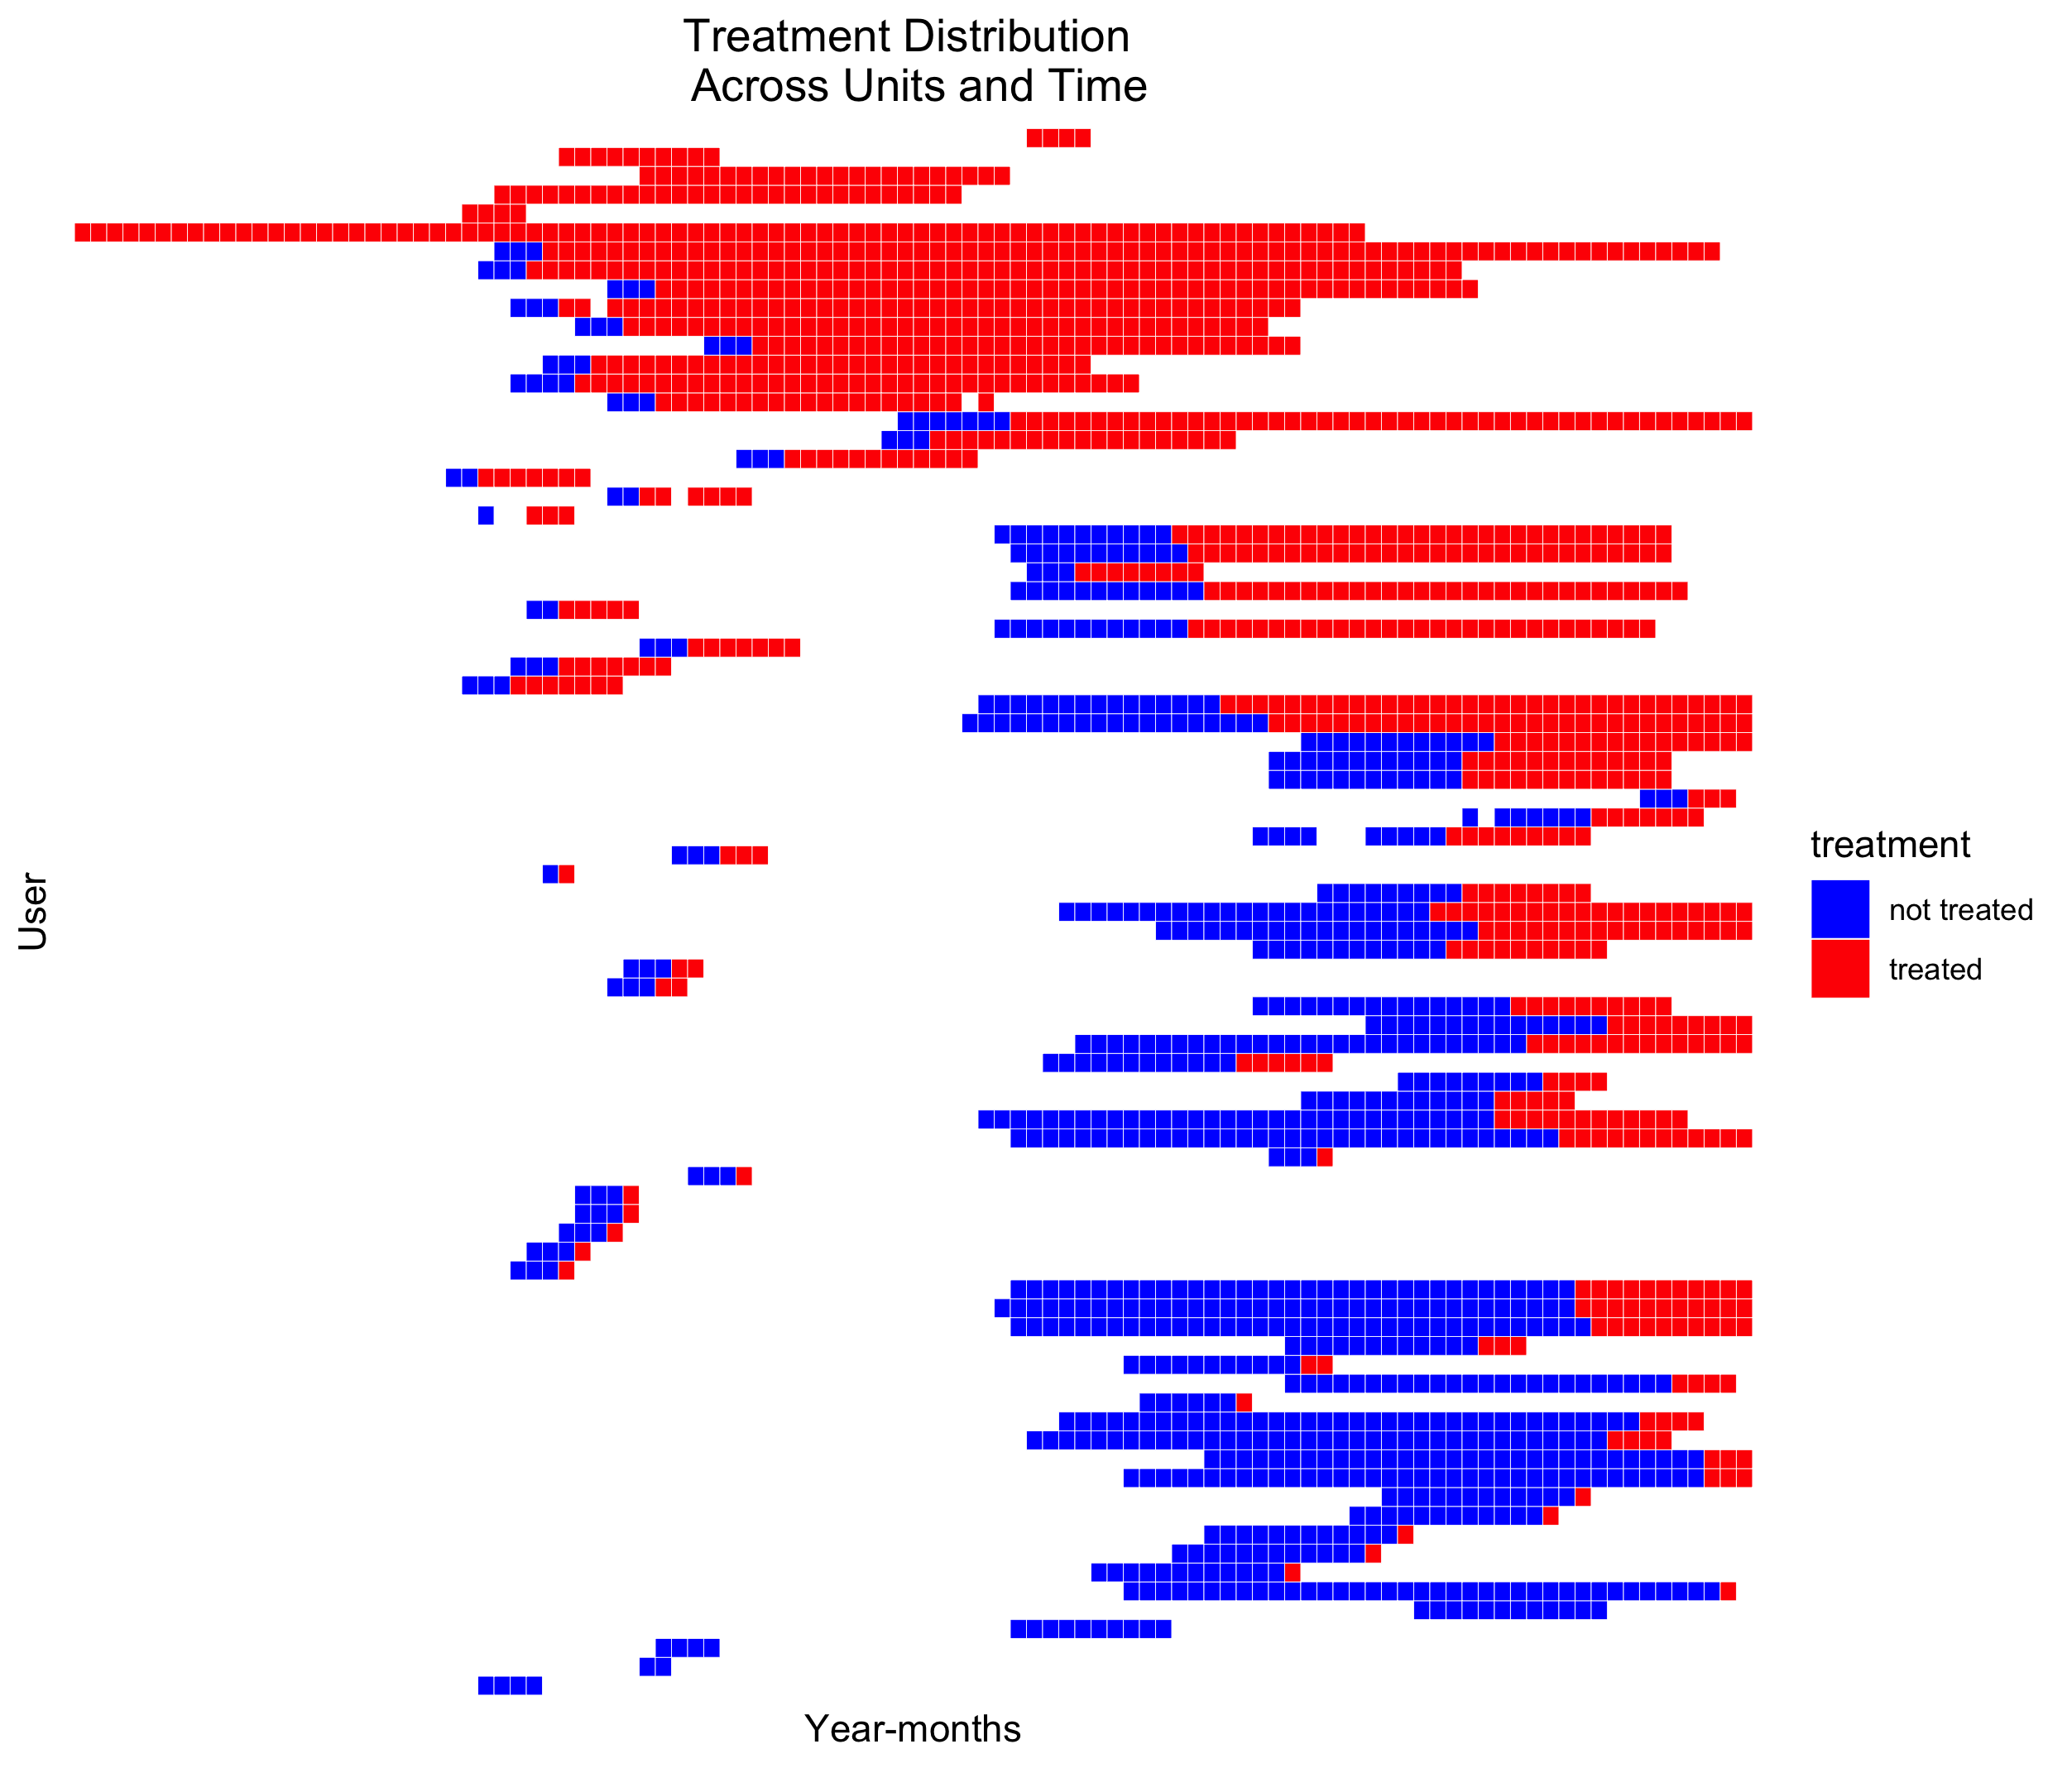
\includegraphics[width=0.8\linewidth]{\figdir/treatplot_sample_raw.png}
\label{fig:treatplot}
\fignote{\textwidth}{Each horizontal line shows the observed pre and post
    signup periods in blue and red, respectively, for one of 200 randomly
    selected users. The faint vertical white lines indicate month borders,
    whitespace indicates periods in which we do not observe the user. To
the left of the observed period, this is because the app cannot access data
before that point when the user signs up; to the right, because they have
stopped using the app.}
\end{figure}

Figure~\ref{fig:treatplot} shows how we can leverage
pre-signup data provided in the MDB data to construct valid control groups.
Each row of cells shows data for one of 200 randomly selected users, with red
cells indicating data from pre-signup months and blue cells indicating data
from post-signup months. Signup thus occured sometime during the first blue
coloured month, and we can use users who have not yet signed up (whose cells
are still red) as a comparison group.


\paragraph{Estimation:}%
\label{par:estimation_}

$ATT(g,t)$ can be estimated by replacing expectations with their sample
analogues,

\begin{equation}
    \widehat{ATT(g,t)} = \frac{1}{N_g}\sum_{i:G_i=g}[Y_{i,t} - Y_{i, g-1}] -
    \frac{1}{N_\mathcal{G}}\sum_{i:G_i \in \mathcal{G}}[Y_{i,t} - Y_{i, g-1}].
\end{equation}

Once these building blocks are estimated, aggregating them to event-study type treatment effects that provide the (weighted)
average treatment effect $l$ periods away from treatment adoption across
different adoption groups can be achieved by calculating

\begin{equation}
    \label{eq:att_es}
    ATT_l = \sum_g w_gATT(g,g+l),
\end{equation}

\noindent where $w_g = P(G = g | g \in \mathcal{G})$ are the groups relative frequencies in the
treated population. When calculating these event study parameters, I use a
panel balanced in event times, with all units being observed for at least 5
treatment periods. This avoids the $ATT_l$ being influenced by different
group compositions at different periods $l$.\footnote{See Section 3.1.1 in
\citet{callaway2021difference} for a more detailed discussion.}


\paragraph{Inference:}%
\label{par:inference_}

Inference is based on a bootstrap proceedure that can account for clustering
and produces simultaneous (or uniform) confidence bands that account for
multiple hypothesis testing.\footnote{For more details on the inference
    proceedure, see Section 4.1 in \citet{callaway2021difference}. The
    interpretation of uniform and pointwise confidence intervals differ in the
    following way: a uniform 95\% confidence band accounts for multiple
    hypothesis testing in that it is constructed such that \textit{all} shown
    coefficients cover their corresponding true value 95 percent of the time.
    In contrast, a more commonly used pointwise 95\% confidence band is
    constructed such that the confidence interval for each parameter covers the
true parameter 95 percent of the time.} 




